\newcommand{\NWtarget}[2]{#2}
\newcommand{\NWlink}[2]{#2}
\newcommand{\NWtxtMacroDefBy}{Fragment defined by}
\newcommand{\NWtxtMacroRefIn}{Fragment referenced in}
\newcommand{\NWtxtMacroNoRef}{Fragment never referenced}
\newcommand{\NWtxtDefBy}{Defined by}
\newcommand{\NWtxtRefIn}{Referenced in}
\newcommand{\NWtxtNoRef}{Not referenced}
\newcommand{\NWtxtFileDefBy}{File defined by}
\newcommand{\NWtxtIdentsUsed}{Uses:}
\newcommand{\NWtxtIdentsNotUsed}{Never used}
\newcommand{\NWtxtIdentsDefed}{Defines:}
\newcommand{\NWsep}{${\diamond}$}
\newcommand{\NWnotglobal}{(not defined globally)}
\newcommand{\NWuseHyperlinks}{}
\documentclass{article}
\usepackage{hyperref}
\usepackage{graphicx}
\renewcommand{\NWtarget}[2]{\hypertarget{#1}{#2}}
\renewcommand{\NWlink}[2]{\hyperlink{#1}{#2}}
\title{Slot Machine}
\author{Soham}
\begin{document}
\maketitle

\section{Specification}
User gamble with Money which Casino provides them. User inputs the bet amount and they they hit the deal button to spin the seven bars displaying the symbols.
The Machine comes up with a random sequence of predecided symbols.
Calculating the amount that a user wins in one spin, it adds that no. of coins to their total coins.
The gambling further continues until the user wants to quite or he/she runs out of coins.




\section{Analysis/Design}
Gambler will be provided with 100 credit(coins) initially, and will be given the option to adjust the bet. They can either bet 1 coin, 5 coins, 10 coins, or 25 coins to adjust their bets. Bet amount will be deducted from their total credits as they hit the Spin button.\\

As the user hits the spin button, 5 symbols will be displayed. The sequence of symbols will thus determine the amount(credit) the user earns in that round. \\

There would be total of 10 symbols that can be used to display the sequence.\\

Determining the number of winnig credit.

\begin{itemize}
\item If all symbols are alike, then add bet\times1000 to the total credits.
\item If no symbol is repeated, then add bet\times500 to the total credits.
\item If a symbol repeats 4 times, then add bet\time100 to the total credits.
\item If the special sequence appears, then add bet\times750 to the total credits.
\item if semi-special sequence appears of four symbols, then add bet\time 50 to the total credits.
\end{itemize}

A User can any time quite to walk away with the credits he/she earned or the ptogram will be terminated as the total credit becomes less then 5.\\ \\

Managin the Program:
\begin{itemize}
\item Initializing the credits to 100 and bet to 0.
\item take input from user to (via buttons) to set their bet until user hits Spin button.
\item Spin button generates a sequence of 7 symbols and display.
\item Read the sequence to determine the credits user won.
\item Change the credits accordingly.
\item Repeat until user hits the quite button.
\end{itemize}




\section{Implementation}
\begin{flushleft} \small
\begin{minipage}{\linewidth}\label{scrap1}\raggedright\small
\NWtarget{nuweb2a}{} \verb@"sm.cpp"@\nobreak\ {\footnotesize {2a}}$\equiv$
\vspace{-1ex}
\begin{list}{}{} \item
\mbox{}\verb@@\\
\mbox{}\verb@@\hbox{$\langle\,${\it Include files}\nobreak\ {\footnotesize \NWlink{nuweb4b}{4b}}$\,\rangle$}\verb@@\\
\mbox{}\verb@@\hbox{$\langle\,${\it Constants}\nobreak\ {\footnotesize \NWlink{nuweb4c}{4c}}$\,\rangle$}\verb@@\\
\mbox{}\verb@@\hbox{$\langle\,${\it Function callback}\nobreak\ {\footnotesize \NWlink{nuweb4a}{4a}}$\,\rangle$}\verb@@\\
\mbox{}\verb@int main()@\\
\mbox{}\verb@{@\\
\mbox{}\verb@@\\
\mbox{}\verb@@\hbox{$\langle\,${\it Create main window}\nobreak\ {\footnotesize \NWlink{nuweb2b}{2b}}$\,\rangle$}\verb@@\\
\mbox{}\verb@@\hbox{$\langle\,${\it Create Widgets for input and output and button}\nobreak\ {\footnotesize \NWlink{nuweb3a}{3a}}$\,\rangle$}\verb@@\\
\mbox{}\verb@@\hbox{$\langle\,${\it Register a callback function to be called when button is pressed}\nobreak\ {\footnotesize \NWlink{nuweb3b}{3b}}$\,\rangle$}\verb@@\\
\mbox{}\verb@@\hbox{$\langle\,${\it Show window with its controls}\nobreak\ {\footnotesize \NWlink{nuweb3c}{3c}}$\,\rangle$}\verb@@\\
\mbox{}\verb@return(Fl::run());@\\
\mbox{}\verb@ @\\
\mbox{}\verb@}@\\
\mbox{}\verb@@{\NWsep}
\end{list}
\vspace{-1.5ex}
\footnotesize
\begin{list}{}{\setlength{\itemsep}{-\parsep}\setlength{\itemindent}{-\leftmargin}}

\item{}
\end{list}
\end{minipage}\vspace{4ex}
\end{flushleft}
% Definitons of functions go here; each in their own macro

\begin{flushleft} \small
\begin{minipage}{\linewidth}\label{scrap2}\raggedright\small
\NWtarget{nuweb2b}{} $\langle\,${\it Create main window}\nobreak\ {\footnotesize {2b}}$\,\rangle\equiv$
\vspace{-1ex}
\begin{list}{}{} \item
\mbox{}\verb@@\\
\mbox{}\verb@Fl_Window* w = new Fl_Window(width,height);@\\
\mbox{}\verb@@{\NWsep}
\end{list}
\vspace{-1.5ex}
\footnotesize
\begin{list}{}{\setlength{\itemsep}{-\parsep}\setlength{\itemindent}{-\leftmargin}}
\item \NWtxtMacroRefIn\ \NWlink{nuweb2a}{2a}.

\item{}
\end{list}
\end{minipage}\vspace{4ex}
\end{flushleft}
Need to pass in XY coordinate (upper left corner) of box, and width, height, and label.
\begin{flushleft} \small
\begin{minipage}{\linewidth}\label{scrap3}\raggedright\small
\NWtarget{nuweb3a}{} $\langle\,${\it Create Widgets for input and output and button}\nobreak\ {\footnotesize {3a}}$\,\rangle\equiv$
\vspace{-1ex}
\begin{list}{}{} \item
\mbox{}\verb@@\\
\mbox{}\verb@Widgets widgets;@\\
\mbox{}\verb@w->begin();@\\
\mbox{}\verb@@\\
\mbox{}\verb@widgets.credit = new Fl_Output(100,75,150,30,"CREDITS:");@\\
\mbox{}\verb@widgets.bet = new Fl_Output(35,350,100,25,"Bet");@\\
\mbox{}\verb@widgets.credit_earned = new Fl_Output(250,350,100,25,"Credits Earned");@\\
\mbox{}\verb@Fl_Button* button_withdraw = new Fl_Button(480,450,160,30,"Withdraw");@\\
\mbox{}\verb@Fl_Button* button_spin = new Fl_Button(470,350,130,30,"Spin");@\\
\mbox{}\verb@Fl_Button* button_bet_again = new Fl_Button(470,300,130,30,"Bet Again");@\\
\mbox{}\verb@Fl_Button* button1 = new Fl_Button(170,400,100,30,"5 Credits");@\\
\mbox{}\verb@Fl_Button* button2 = new Fl_Button(270,400,100,30,"10 Credits");@\\
\mbox{}\verb@Fl_Button* button3 = new Fl_Button(370,400,100,30,"20 Credits");@\\
\mbox{}\verb@Fl_Button* buttonreset = new Fl_Button(50,400,100,30,"Reset");@\\
\mbox{}\verb@Fl_Button* buttonmax = new Fl_Button(490,400,100,30,"Bet Max");@\\
\mbox{}\verb@w->end();@\\
\mbox{}\verb@@{\NWsep}
\end{list}
\vspace{-1.5ex}
\footnotesize
\begin{list}{}{\setlength{\itemsep}{-\parsep}\setlength{\itemindent}{-\leftmargin}}
\item \NWtxtMacroRefIn\ \NWlink{nuweb2a}{2a}.

\item{}
\end{list}
\end{minipage}\vspace{4ex}
\end{flushleft}
\begin{flushleft} \small
\begin{minipage}{\linewidth}\label{scrap4}\raggedright\small
\NWtarget{nuweb3b}{} $\langle\,${\it Register a callback function to be called when button is pressed}\nobreak\ {\footnotesize {3b}}$\,\rangle\equiv$
\vspace{-1ex}
\begin{list}{}{} \item
\mbox{}\verb@@\\
\mbox{}\verb@button_withdraw->callback(button_clicked,&widgets);@\\
\mbox{}\verb@button_spin->callback(button_clicked,&widgets);@\\
\mbox{}\verb@button_bet_again->callback(button_clicked,&widgets);@\\
\mbox{}\verb@button1->callback(button_clicked,&widgets);@\\
\mbox{}\verb@button2->callback(button_clicked,&widgets);@\\
\mbox{}\verb@button3->callback(button_clicked,&widgets);@\\
\mbox{}\verb@buttonreset->callback(button_clicked,&widgets);@\\
\mbox{}\verb@buttonmax->callback(button_clicked,&widgets);@\\
\mbox{}\verb@@{\NWsep}
\end{list}
\vspace{-1.5ex}
\footnotesize
\begin{list}{}{\setlength{\itemsep}{-\parsep}\setlength{\itemindent}{-\leftmargin}}
\item \NWtxtMacroRefIn\ \NWlink{nuweb2a}{2a}.

\item{}
\end{list}
\end{minipage}\vspace{4ex}
\end{flushleft}
\begin{flushleft} \small
\begin{minipage}{\linewidth}\label{scrap5}\raggedright\small
\NWtarget{nuweb3c}{} $\langle\,${\it Show window with its controls}\nobreak\ {\footnotesize {3c}}$\,\rangle\equiv$
\vspace{-1ex}
\begin{list}{}{} \item
\mbox{}\verb@@\\
\mbox{}\verb@w->show();@\\
\mbox{}\verb@@{\NWsep}
\end{list}
\vspace{-1.5ex}
\footnotesize
\begin{list}{}{\setlength{\itemsep}{-\parsep}\setlength{\itemindent}{-\leftmargin}}
\item \NWtxtMacroRefIn\ \NWlink{nuweb2a}{2a}.

\item{}
\end{list}
\end{minipage}\vspace{4ex}
\end{flushleft}
These are the declarations of functions called in this program
\begin{flushleft} \small
\begin{minipage}{\linewidth}\label{scrap6}\raggedright\small
\NWtarget{nuweb4a}{} $\langle\,${\it Function callback}\nobreak\ {\footnotesize {4a}}$\,\rangle\equiv$
\vspace{-1ex}
\begin{list}{}{} \item
\mbox{}\verb@@\\
\mbox{}\verb@void button_clicked(Fl_Widget* o, void* v)@\\
\mbox{}\verb@{@\\
\mbox{}\verb@static int bet_counter=0;@\\
\mbox{}\verb@Widgets* w = static_cast<Widgets*>(v);@\\
\mbox{}\verb@bet_counter+=5;@\\
\mbox{}\verb@w->out;@\\
\mbox{}\verb@}@\\
\mbox{}\verb@@{\NWsep}
\end{list}
\vspace{-1.5ex}
\footnotesize
\begin{list}{}{\setlength{\itemsep}{-\parsep}\setlength{\itemindent}{-\leftmargin}}
\item \NWtxtMacroRefIn\ \NWlink{nuweb2a}{2a}.

\item{}
\end{list}
\end{minipage}\vspace{4ex}
\end{flushleft}
These are the include files needed for library function calls
\begin{flushleft} \small
\begin{minipage}{\linewidth}\label{scrap7}\raggedright\small
\NWtarget{nuweb4b}{} $\langle\,${\it Include files}\nobreak\ {\footnotesize {4b}}$\,\rangle\equiv$
\vspace{-1ex}
\begin{list}{}{} \item
\mbox{}\verb@@\\
\mbox{}\verb@#include <iostream>@\\
\mbox{}\verb@using namespace std;@\\
\mbox{}\verb@#include<fl/fl.h>@\\
\mbox{}\verb@#include<fl/fl_window.h>@\\
\mbox{}\verb@#include<fl/fl_button.h>@\\
\mbox{}\verb@#include<fl/fl_output.h>@\\
\mbox{}\verb@@{\NWsep}
\end{list}
\vspace{-1.5ex}
\footnotesize
\begin{list}{}{\setlength{\itemsep}{-\parsep}\setlength{\itemindent}{-\leftmargin}}
\item \NWtxtMacroRefIn\ \NWlink{nuweb2a}{2a}.

\item{}
\end{list}
\end{minipage}\vspace{4ex}
\end{flushleft}
These are the values that will not change during program execution
\begin{flushleft} \small
\begin{minipage}{\linewidth}\label{scrap8}\raggedright\small
\NWtarget{nuweb4c}{} $\langle\,${\it Constants}\nobreak\ {\footnotesize {4c}}$\,\rangle\equiv$
\vspace{-1ex}
\begin{list}{}{} \item
\mbox{}\verb@@\\
\mbox{}\verb@@\\
\mbox{}\verb@const int width = 640;@\\
\mbox{}\verb@const int height = 480;@\\
\mbox{}\verb@struct Widgets@\\
\mbox{}\verb@{@\\
\mbox{}\verb@Fl_Output* out;@\\
\mbox{}\verb@Fl_Output* credit;@\\
\mbox{}\verb@Fl_Output* credit_earned;@\\
\mbox{}\verb@Fl_Output* bet;@\\
\mbox{}\verb@};@\\
\mbox{}\verb@@\\
\mbox{}\verb@@{\NWsep}
\end{list}
\vspace{-1.5ex}
\footnotesize
\begin{list}{}{\setlength{\itemsep}{-\parsep}\setlength{\itemindent}{-\leftmargin}}
\item \NWtxtMacroRefIn\ \NWlink{nuweb2a}{2a}.

\item{}
\end{list}
\end{minipage}\vspace{4ex}
\end{flushleft}
\section{Test}
%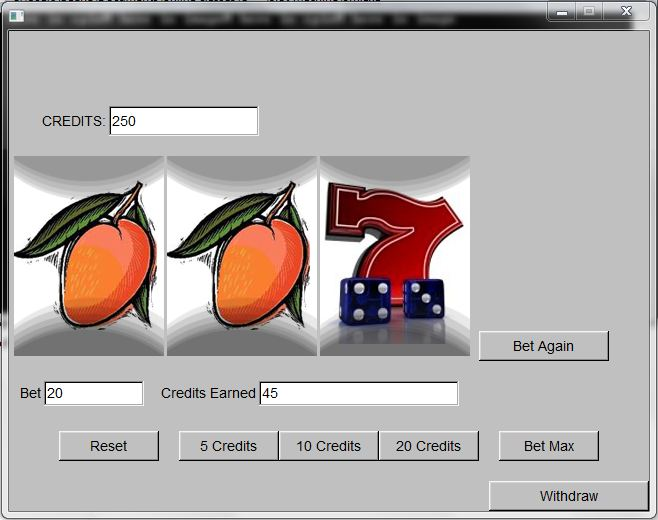
\includegraphics[scale=0.5]{lab.jpg}
\end{document}

